\scanpage{52}
\mspage{\unsure{6}}
Je vais introduire, dans la sphère $\widetilde\Sigma$ dont le degré de connexion est 0, cinq ouverts, pris aussi grands que possible, qui soient simplement connexes -- obtenus en pratiquant des ``coupures'' qui relient entre eux les \deleted{trois} bords $U_i$ des trois ``trous'' \deleted{$\unsure{\Sigma}$}. On pose
\figure{
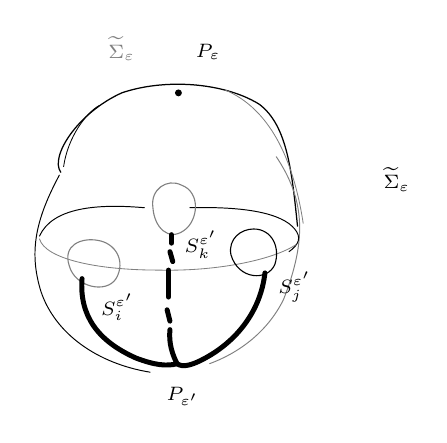
\begin{tikzpicture}[x=.018cm,y=-.018cm,every node/.style={font=\scriptsize},line cap=round,line join=round]
\draw[line width=.45pt] (33,130) .. controls (25,119) and (45,88) .. (76,74) .. controls (105,64) and (147,66) .. (173,82) .. controls (193,97) and (196,130) .. (200,168);
\draw[line width=.35pt] (32,132) .. controls (16,162) and (10,185) .. (19,214) .. controls (29,244) and (59,265) .. (96,271);
\draw[line width=.35pt,gray] (185,119) .. controls (205,149) and (207,177) .. (190,220) .. controls (178,244) and (157,258) .. (138,265);
\draw[line width=.3pt] (35,126) .. controls (38,105) and (51,88) .. (60,83);
\draw[line width=.3pt,gray] (149,72) .. controls (180,85) and (197,120) .. (204,166);
\draw[line width=.35pt] (18,175) .. controls (27,155) and (58,152) .. (92,155);
\draw[line width=.35pt] (124,155) .. controls (164,154) and (189,159) .. (198,170) .. controls (203,176) and (201,181) .. (194,186);
\draw[line width=.3pt,gray] (18,177) .. controls (22,191) and (58,199) .. (102,199) .. controls (146,200) and (184,191) .. (199,181);
\draw[line width=.4pt,gray] (39,196) .. controls (34,181) and (48,176) .. (59,178) .. controls (72,180) and (79,193) .. (72,205) .. controls (65,216) and (43,211) .. (39,196);
\draw[line width=.4pt,gray] (98,155) .. controls (96,142) and (108,134) .. (118,139) .. controls (132,144) and (130,164) .. (120,171) .. controls (109,179) and (99,169) .. (98,155);
\draw[line width=.4pt] (153,188) .. controls (151,177) and (160,170) .. (169,170) .. controls (182,170) and (188,183) .. (184,195) .. controls (179,207) and (158,206) .. (153,188);
\draw[line width=1.8pt] (48,205) .. controls (46,231) and (59,249) .. (86,261) .. controls (99,266) and (108,267) .. (115,265);
\draw[line width=1.8pt] (177,201) .. controls (174,228) and (157,249) .. (135,261) .. controls (126,266) and (119,268) .. (115,265);
\draw[line width=1.8pt] (111,174)--(111,180);
\draw[line width=1.8pt] (110,186)--(112,193);
\draw[line width=1.8pt] (109,199)--(109,218);
\draw[line width=1.8pt] (108,227)--(110,235);
\draw[line width=1.8pt] (110,241) .. controls (109,251) and (112,259) .. (115,265);
\fill (116,74) circle[radius=1.25pt];
\node[gray] at (76,43) {$\widetilde\Sigma_\varepsilon$};
\node at (137,45) {$P_\varepsilon$};
\node at (119,288) {$P_{\varepsilon'}$};
\node at (73,225) {$S_i^{\varepsilon'}$};
\node at (132,181) {$S_k^{\varepsilon'}$};
\node at (198,211) {$S_j^{\varepsilon'}$};
\node at (270,135) {$\widetilde\Sigma_\varepsilon$};
\end{tikzpicture}
}
\[
(27)\quad\left\{\begin{aligned}
\widetilde\Sigma_\varepsilon&=\widetilde\Sigma\setminus\bigcup_{i\in J}\operatorname{supp}d_i^\varepsilon \qquad\varepsilon\in\uline{\varepsilon}\\
\widetilde\Sigma_i&=\widetilde\Sigma\setminus\bigcup_{\substack{j\in J\setminus\{i\}\\\deleted{\omega\in\unsure{\uline{\omega}|\omega}}}}\deleted{\operatorname{supp}}b_i^{\unsure{\deleted{\omega}|\omega}}
\end{aligned}\right.
\]
\margin{(où $b_i=\operatorname{supp}\widetilde b_i^\omega$\newline
\deleted{$=\operatorname{supp}\unsure{c_i^\omega|b_i^\omega}\cup\operatorname{supp}\unsure{c_i^{\omega'}|b_i^{\omega'}}$}\newline
$=\operatorname{supp}c_i^\omega\cup\operatorname{supp}c_i^{\omega'}$)}
\figure{
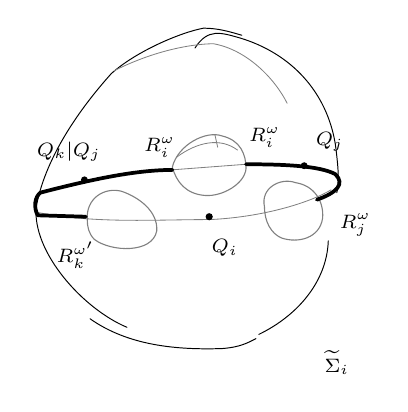
\begin{tikzpicture}[x=.018cm,y=-.018cm,every node/.style={font=\scriptsize},line cap=round,line join=round]
\draw[line width=.35pt] (73,46) .. controls (47,75) and (26,108) .. (20,140) .. controls (17,172) and (53,212) .. (84,225);
\draw[line width=.35pt] (58,219) .. controls (85,238) and (119,241) .. (151,240) .. controls (164,239) and (169,236) .. (175,233);
\draw[line width=.35pt] (132,28) .. controls (141,14) and (150,17) .. (164,21) .. controls (200,32) and (225,59) .. (231,96) .. controls (233,111) and (234,124) .. (232,130);
\draw[line width=.35pt] (226,164) .. controls (225,193) and (204,217) .. (177,230);
\draw[line width=.35pt] (73,46) .. controls (91,30) and (122,17) .. (138,14) .. controls (149,14) and (158,17) .. (165,19);
\draw[line width=.3pt,gray] (75,44) .. controls (107,28) and (134,25) .. (145,25) .. controls (168,29) and (188,49) .. (197,67);
\draw[line width=.3pt,gray] (21,144) .. controls (62,152) and (104,149) .. (143,149) .. controls (183,147) and (215,136) .. (228,128);
\draw[line width=.3pt,gray] (115,114)--(168,110);
\draw[line width=.4pt,gray] (56,149) .. controls (55,134) and (68,126) .. (80,129) .. controls (92,133) and (106,143) .. (105,157) .. controls (102,173) and (73,172) .. (61,163) .. controls (57,159) and (56,154) .. (56,149);
\draw[line width=.4pt,gray] (116,112) .. controls (120,96) and (140,86) .. (151,90) .. controls (164,93) and (168,103) .. (168,113) .. controls (167,124) and (151,133) .. (139,132) .. controls (126,131) and (119,123) .. (116,112);
\draw[line width=.3pt,gray] (119,105) .. controls (134,94) and (150,91) .. (162,100);
\draw[line width=.3pt,gray] (146,89)--(148,98);
\draw[line width=.4pt,gray] (181,140) .. controls (178,127) and (192,119) .. (203,123) .. controls (216,125) and (223,136) .. (222,148) .. controls (220,162) and (205,166) .. (193,162) .. controls (186,159) and (181,151) .. (181,140);
\draw[line width=1.35pt] (116,114) .. controls (88,114) and (54,122) .. (23,130) .. controls (19,133) and (18,140) .. (21,146)--(55,147);
\draw[line width=1.35pt] (168,110) .. controls (194,110) and (220,111) .. (231,117) .. controls (238,124) and (232,130) .. (218,135);
\fill (54,121) circle[radius=1.25pt];
\fill (142,147) circle[radius=1.3pt];
\fill (209,111) circle[radius=1.25pt];
\node at (43,101) {$\unsure{Q_k|Q_j}$};
\node at (227,94) {$Q_j$};
\node at (153,169) {$Q_i$};
\node at (107,98) {$R_i^\omega$};
\node at (181,91) {$R_i^\omega$};
\node at (48,174) {$R_k^{\omega'}$};
\node at (245,153) {$R_j^\omega$};
\node at (232,250) {$\widetilde\Sigma_i$};
\end{tikzpicture}
}
Ce sont bien des ouverts \deleted{de $\unsure{\overline{\Sigma}|\widetilde{\Sigma}}$} simplement connexes de la sphère à trous $\widetilde\Sigma$ (car le \inserted{\unsure{connexe|connexes} et à} \unsure{complémentaire|complémentaires} est connexe. On dit que $P_\omega$ est le \uline{centre} de $\widetilde\Sigma_\omega$, $Q_i$ le \uline{centre} de $\widetilde\Sigma_i$.
\margin{ce sont des ouverts denses, et pour cette raison connexes}
On pose
\[
(28)\quad\left\{\begin{aligned}
\Pi_{\unsure{\varepsilon}}&=\Pi_1(\widetilde\Sigma,\widetilde\Sigma_\varepsilon)\simeq\Pi_1(\Sigma^*,\Sigma_{\unsure{\varepsilon}}^*)\simeq\Pi_1(\Sigma^*,P_{\unsure{\varepsilon}})\\
\Pi_i&=\Pi_1(\widetilde\Sigma,\widetilde\Sigma_i)=\Pi_1(\Sigma^*,\Sigma_i^*)\simeq\Pi_1(\Sigma^*,Q_i)
\end{aligned}\right.
\]
en faisant les identifications indiquées par ces formules. \deleted{\unsure{De}} Pour $\forall\ x\in\widetilde\Sigma_\omega$ resp $x\in\widetilde\Sigma_i$, on pose
\[
(29)\quad\left\{\begin{aligned}
\varphi_{\varepsilon,x}\text{ ou }\varphi_\omega&:\Pi_\varepsilon\xrightarrow{\sim}\Pi_1(\widetilde\Sigma,x)\quad\left(\begin{gathered}\simeq\Pi_1(\Sigma^*,x)\text{ si}\\x\in\Sigma^*\end{gathered}\right)\\
\text{resp. }\varphi_{i,x}\text{ ou }\varphi_i&:\Pi_i\xrightarrow{\sim}\Pi_1(\widetilde\Sigma,x)\qquad\text{--}
\end{aligned}\right.
\]
\margin{Les $\varphi$ sont appelés \uline{isom} \uline{de} \uuline{transition}}
\margin{51}
